\newpage
\subsubsection{UC5 - Configurazione del plug-in per la predizione}
\label{sssec:uc5}

\begin{figure}[h!]
  \begin{center}
    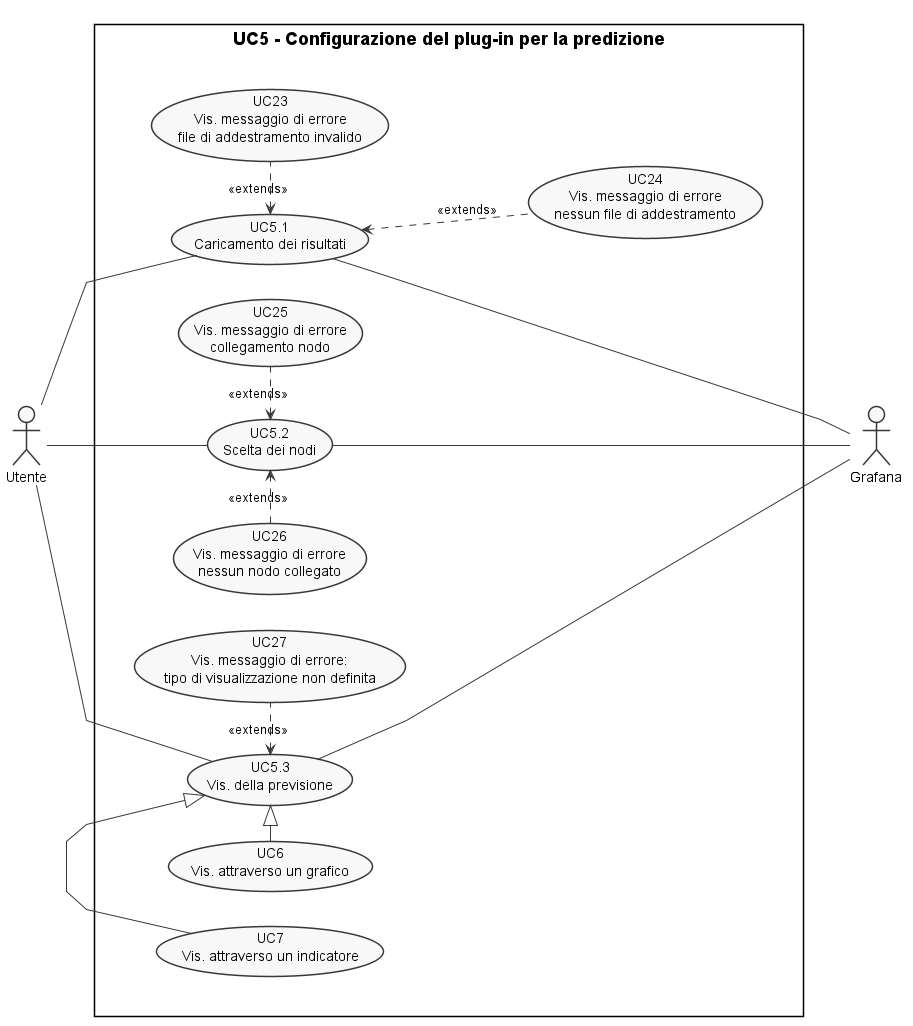
\includegraphics[width=18cm]{uc5.png}\\
    \caption{UC5 - Configurazione del plug-in per la predizione}%
    \label{fig:uc3}
  \end{center}
  \end{figure}

  \begin{itemize}
    \item \textbf{Attore primario}: Utente;
    \item \textbf{Attore secondario}: Grafana;
    \item \textbf{Descrizione}: Configurazione del plug-in per ottenere le previsioni;
    \item \textbf{Precondizione}: L'utente ha abilitato il plug-in e si trova nella pagina di configurazione;
    \item \textbf{Scenario principale}:
    \begin{enumerate}
      \item L'utente carica il file JSON contente i risultati dell'addestramento (UC5.1);
      \item L'utente sceglie su quali nodi fare le previsioni (UC5.2);
    \end{enumerate}
    \item \textbf{Postcondizione}: L'utente ha configurato il plug-in, il quale diventa pronto per essere avviato.
  \end{itemize}

\paragraph{UC5.1 - Caricamento risultati}
\label{para:uc5.1}
\begin{itemize}
  \item \textbf{Attore primario}: Utente;
  \item \textbf{Attore secondario}: Grafana;
  \item \textbf{Descrizione}: L'utente carica il file JSON contenente i risultati ottenuti dall'addestramento;
  \item \textbf{Precondizione}: Il sistema permette di leggere un file JSON, l'utente ha a disposizione un file con all'interno i risultati (UC1.5);
  \item \textbf{Scenario principale}: Vengono caricati i risultati dell'addestramento presenti in un file JSON;
  \item \textbf{Postcondizione}: Vengono caricati i risultati dell'addestramento avvenuto precedentemente e salvati in un file JSON;
  \item \textbf{Estensioni}:
  \begin{enumerate}
    \item UC5.1 viene esteso nel caso d'uso UC23 con la visualizzazione del messaggio di errore quando viene fornito un predittore in un formato non valido;
    \item UC5.1 viene esteso nel caso d'uso UC24 con la visualizzazione del messaggio di errore quando l'utente non inserisce alcun file per l'addestramento.
    \end{enumerate}
\end{itemize}

\paragraph{UC5.2 - Scelta dei nodi}
\label{para:uc5.2}
\begin{itemize}
  \item \textbf{Attore primario}: Utente;
  \item \textbf{Attore secondario}: Grafana;
  \item \textbf{Descrizione}: L'utente sceglie su che nodi effettuare la previsione;
  \item \textbf{Precondizione}: L'utente ha caricato il file con i dati di addestramento (UC5.1);
  \item \textbf{Scenario principale}: L'utente, data una lista di nodi, seleziona su quali vuole ottenere la predizione;
  \item \textbf{Postcondizione}: L'utente ha selezionato su che nodi effettuare la predizione;
  \item \textbf{Estensioni}:
  \begin{enumerate}
    \item UC5.1 viene esteso nel caso d'uso UC25 con la visualizzazione del messaggio di errore quando non viene selezionato nessun nodo valido;
    \item UC5.1 viene esteso nel caso d'uso UC26 con la visualizzazione del messaggio di errore quando non viene selezionato alcun nodo.
    \end{enumerate}
\end{itemize}


